\documentclass{beamer}
\usepackage{presentation}
\title{Generalizing Lenses}
\subtitle{A New Foundation for Bidirectional Programming}
\author{Daniel Wagner} % for hyperref
\date{June 13, 2014}

\begin{document}

\author{Daniel Wagner\\[3ex]
\includegraphics[width=0.2\linewidth]{images/plclub-logo.pdf}} % for beamer
\maketitle

\begin{frame}
    \frametitle{Bidirectional programming}
    Keep two pieces of data in synch. It's a common problem.

    Don't want to write two programs for maintenance reasons.
\end{frame}

\begin{frame}
    \frametitle{Databases}
    First interest was in the database community, via view-update problem.

    Generated idea of constant-complement updating.

    Basis for asymmetric lenses. Lots of language-based research followup.
\end{frame}

\begin{frame}
    \frametitle{UI}
    Separate research thread on user interfaces.

    Constraints between interface elements (e.g. when selecting a range, the
    upper bound is above the lower bound). But don't want to constrain user.

    So restore broken constraints. Led to constraint maintainers.
\end{frame}

\begin{frame}
    \frametitle{Dissatisfaction}
    Basic assumption of asymmetric lenses: source contains all data. View
    contains some chunk of interest to the user.

    Behavioral laws not strong enough.

    Surprisingly hard problem: alignment.

    Need modularity.
\end{frame}

\begin{frame}
    \frametitle{Symmetric lenses}
    First lens framework to support symmetry and address all the issues that
    composition causes -- computability, behavioral equality.

    But behavioral laws are no better, and no improvement on alignment.
\end{frame}

\begin{frame}
    \frametitle{Edit lenses}
    Extend symmetric lenses with explicit alignment handling.

    While we're at it, incremental operation for performance.

    Did an algebraic study of the framework, resulting in a large collection
    of abstract syntax.

    Prototype implementation exploring the problem of generating alignment
    information.
\end{frame}

\begin{frame}
    \frametitle{Related work preview}
    Table proving we are better than everybody else.
\end{frame}

\begin{frame}
    \frametitle{Other models of edits}

    \begin{itemize}
        \item $X \times X$ (before and after)
            \begin{itemize}
                \item State-based lenses
                \item[\ybullet] Very simple starting point
                \item[\nbullet] Not enough information about alignment
            \end{itemize}
        \item $X \to X$ (extensional edit operation)
            \begin{itemize}
                \item Stevens' algebraic study of delta lenses
                \item[\ybullet] Models many behaviors
                \item[\nbullet] Difficult to recover intensional data
            \end{itemize}
        \item category on $X$ (collection of edits for each before/after
            pair)
            \begin{itemize}
                \item Diskin, et al's delta lenses
                \item[\ybullet] Very rich information about change
                \item[\nbullet] Very rich information about change
            \end{itemize}
    \end{itemize}
\end{frame}

\begin{frame}
    \frametitle{Modules}
    Keep the best features of each: collection of edits for easy
    introspection + mapping to functions to cover many behaviors.

    \vpause

    Module $\left<X,\DX,\odot_X,\init_X\right>$ is:
    \begin{itemize}
        \item Set of values to be edited $X$
        \item Monoid of edits $\DX$
        \item Homomorphism from edits to operations $\odot_X \in \DX \to X
            \partialto X$
        \item Default value $\init_X$ is a technical detail; explanation
            later
    \end{itemize}
\end{frame}

\begin{frame}
    \frametitle{Monoids}
    Quick review: monoid means
    \begin{itemize}
        \item There is an identity $\ONE$
        \item and an associative binary operation (juxtaposition).
    \end{itemize}

    Homomorphisms $f$ respect this structure.
    \[f(\ONE) = \ONE\]
    \[f(m\;n) = f(m)\;f(n)\]
    In particular, for edits: identity always succeeds and does nothing, and
    edits can be run in sequence.
\end{frame}

\begin{frame}
    \frametitle{Partiality}
    \[\odot_X \in \DX \to \alert<2>{X \partialto X}\]

    \pause\pause

    Requiring totality forces you to include unnatural edits.

    \[M \triangleq \{\ONE\} \cup \{a \mapsto b \mid a,b \in \N\}\]

    With totality:
    \begin{align*}
        (a \mapsto b)\;(b \mapsto c) \odot a &= c \\
        (a \mapsto b)\;(b \mapsto c) \odot b &= c
    \end{align*}
    \ldots must expand $M$ to accommodate this.

    With partiality, can define
    \[(a \mapsto b)\;(b \mapsto c) \triangleq a \mapsto c\]

    \pause
    Theorem: Partiality is an illusion.
\end{frame}

\begin{frame}
    \frametitle{Data structures}

    Common approach to implementing complex data structures:

    \[\tau := 0 \mid 1 \mid X \mid \tau+\tau \mid \tau\times\tau
           \mid \fix X\tau {\color<2->{lightgray}\mid \tau\to\tau}\]

    Try to design edit modules for each of these types.

    \vpause

    \uncover<3>{\alert{Does not work well.}}
\end{frame}

\begin{frame}
    \frametitle{Free monoids}
    All modules in this talk based on lists:
    \begin{align*}
        \ONE &\triangleq \left<\right> \\
        \left<a_0,\cdots,a_m\right>\;\left<b_0,\cdots,b_n\right>
            &\triangleq \left<a_0,\cdots,a_m,b_0,\cdots,b_n\right>
    \end{align*}

    Elements are atomic edits, and get run in sequence:
    \[\left<a,b,c\right>\odot x \triangleq
        a \odot\gen (b \odot\gen (c \odot\gen x))\]
\end{frame}

\begin{frame}
    \frametitle{Products}
    % TODO: turn this into a cats and dogs diagram
    How to edit $X \times Y$? Either edit $X$ or edit $Y$.

    \begin{align*}
        \D(X\times Y) &\triangleq \DX + \DY \\
        \mlleft \dx \odot\gen (x,y) &\triangleq (\dx \odot x, y) \\
        \mlright\dy \odot\gen (x,y) &\triangleq (x, \dy \odot y)
    \end{align*}
\end{frame}

\begin{frame}
    \frametitle{Sums}
    Choices are less canonical, and significantly more fiddly.

    \vspace{-2ex}

    % TODO: for dogs, perhaps age them instead of adding an accessory
    \begin{diagram}
        \node[matrix of nodes
             ,ampersand replacement=\&
             ,column sep=8em
             ,nodes={anchor=center}
             ] (pictures) {
                \strut Cats \&
                \strut Dogs \\
                
\includegraphics[width=4em]{images/without_hat.jpg}   \&
                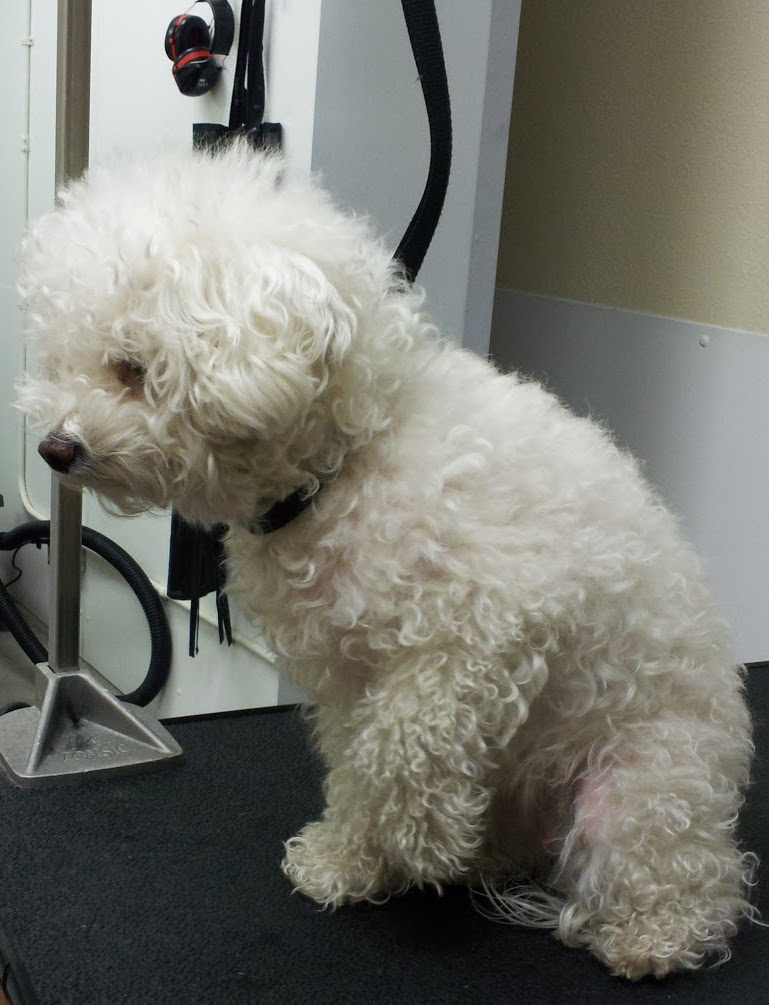
\includegraphics[width=4em]{images/without_scarf.jpg} \\[4ex]
                
\includegraphics[width=4em]{images/with_hat.jpg}      \&
                
\includegraphics[width=4em]{images/with_scarf.jpg}    \\
            }

            ($(pictures-1-1)!.5!(pictures-1-2)$) node (plus) {\strut +}
            (plus |- pictures-3-1.south) node[below]
                {
                    \strut%
                    \only<2>{$\mlstayl{\mbox{+hat}}$}%
                    \only<3>{$\mlstayr{\mbox{+scarf}}$}%
                    \only<4>{$\mlswitchlr\ONE$}%
                    \only<5>{$\mlswitchlr{\mbox{+scarf}}$}%
                    \only<6>{$\mlswitchll\ONE$}%
                }

            (pictures-2-1.west) +(-1.5,0) node (spacer-l) {}
            (pictures-2-2.east) +( 1.5,0) node (spacer-r) {}
            ;

        \path<2>
            (pictures-2-1)     edge[->]                  (pictures-3-1)
            (pictures-3-1.225) edge[->] node {\nbullet} +(-0.5,-0.5)
            (pictures-2-2.315) edge[->] node {\nbullet} +( 0.5,-0.5)
            (pictures-3-2.315) edge[->] node {\nbullet} +( 0.5,-0.5)
            ;
        \path<3>
            (pictures-2-1.225) edge[->] node {\nbullet} +(-0.5,-0.5)
            (pictures-3-1.225) edge[->] node {\nbullet} +(-0.5,-0.5)
            (pictures-2-2)     edge[->]                  (pictures-3-2)
            (pictures-3-2.315) edge[->] node {\nbullet} +( 0.5,-0.5)
            ;
        \path<4>
            (pictures-2-1)     edge[->]                  (pictures-2-2)
            (pictures-3-1)     edge[->]                  (pictures-2-2)
            (pictures-2-2.315) edge[->] node {\nbullet} +( 0.5,-0.5)
            (pictures-3-2.315) edge[->] node {\nbullet} +( 0.5,-0.5)
            ;
        \path<5>
            (pictures-2-1)     edge[->]                  (pictures-3-2)
            (pictures-3-1)     edge[->]                  (pictures-3-2)
            (pictures-2-2.315) edge[->] node {\nbullet} +( 0.5,-0.5)
            (pictures-3-2.315) edge[->] node {\nbullet} +( 0.5,-0.5)
            ;
        \path<6>
            (pictures-2-1)     edge[loop right]          (pictures-2-1)
            (pictures-3-1)     edge[->]                  (pictures-2-1)
            (pictures-2-2.315) edge[->] node {\nbullet} +( 0.5,-0.5)
            (pictures-3-2.315) edge[->] node {\nbullet} +( 0.5,-0.5)
            ;
    \end{diagram}
\end{frame}

\begin{frame}
    \frametitle{Sums, recap}
    Six kinds of sum edit for $X + Y$:
    \begin{center}
        $\mlstayl\dx$

        $\mlswitchll\dx$

        $\mlswitchrl\dx$

        \vspace{2ex}

        $\mlstayr\dy$

        $\mlswitchlr\dy$

        $\mlswitchrr\dy$
    \end{center}
\end{frame}

% TODO: I think can steal some slides explaining why alignment is
% important/hard to put here. Otherwise maybe it's hard to justify why
% ``rewrite the list elements'' isn't a good replacement for ``reorder the
% list'' later.

\begin{frame}
    \frametitle{Recursive types}
    First idea: $\D(\fix X\tau)\simeq\D(\tau[\fix X\tau/X])$.

    For lists with elements from module $A$, i.e. $\fix X1+A \times X$:

    \begin{description}[$\mlstayr{\mlright\dx}$]
        \item[$\mlstayl\anything$] Do nothing to the currently empty list.
        \item[$\mlswitch_{\anything L}(\anything)$] Delete the entire list.
        \item[$\mlstayr{\mlleft{\d a}}$] Modify the head of the list.
        \item[$\mlstayr{\mlright\dx}$] Modify the tail of the list.
        \item[$\mlswitch_{\anything R}(\anything)$] Replace the current
            list.
    \end{description}

    Information never migrates; can't swap list elements.

    \alert{No way to insert or delete in the middle of the list.}

    \pause

    More baroque approaches don't work well either.
\end{frame}

\begin{frame}
    \frametitle{Containers}
    A standard container $\left<I,P\right>$ is
    \begin{itemize}
        \item A set of shapes $I$ and
        \item For each shape $i$, a set $P_i$ of positions.
    \end{itemize}
    An \emph{$X$-instance} $\left<i,f\right>$ of container $\left<I,P\right>$ is
    \begin{itemize}
        \item A shape $i \in I$ and
        \item A function $f \in P_i \to X$.
    \end{itemize}
\end{frame}

\begin{frame}
    \frametitle{Container restrictions}
    Three important changes:

    \begin{itemize}
        \item Module of shape edits
        \item Universe of positions $P_U$
        \item Partial order $\le$ on shapes (with $P$ monotone)
    \end{itemize}
\end{frame}

% TODO: give lists as an example here?
% (could be a good excuse for a diagram break)

\begin{frame}
    \frametitle{Container module}
    \begin{align*}
        \D\left<I,P\right>_X
            \triangleq{}&
                \{\ml{mod}(p,\dx) \mid p \in P_U\}
            \\ \mathrel{\cup}{}&
                \{\ml{ins}(\d i) \mid \d i\;i \ge i\mbox{ whenever defined}\}
            \\ \mathrel{\cup}{}&
                \{\ml{del}(\d i) \mid \d i\;i \le i\mbox{ whenever defined}\}
            \\ \mathrel{\cup}{}&
                \{\ml{swap}(\d i,f) \mid f_i \in P_{\d i\;i} \simeq P_i
                \mbox{ whenever defined} \}
            \\ \mathrel{\cup}{}&
                \{\ml{fail}\}
    \end{align*}
\end{frame}

\begin{frame}
    \frametitle{Container mapping lens}
    The right edit set makes $\ml{map}$ easy.
    \begin{align*}
        \ml{map}(\ell).\dputr\gen(\ml{mod}(p,\dx))
            &\triangleq \ml{mod}(p,\ell.\dputr(\dx)) \\
        \ml{map}(\ell).\dputr\gen(\dv) &\triangleq \dv
    \end{align*}

    % TODO: perhaps should have a second slide with the real implementation,
    % at least just to flash...?
\end{frame}

\begin{frame}
    \frametitle{Alignment}
    Explicit edit instructions simplifies alignment handling.

    Alignment slightly implicit in the edits. But need not be made explicit
    during handling.

    When underlying lens has trivial complement, this has trivial
    complement. (Lenses only make promises about good edits!)
\end{frame}

\begin{frame}
    \frametitle{Reshaping}
    Actually, not so important that source and target containers are the
    same.

    Position bijection $\Rightarrow$ lens. Bijection can even depend on
    state to have some hysteresis.

    Probably needs 2-3 more slides to do the details justice.
\end{frame}

\begin{frame}
    \frametitle{Other results}
    Lens equivalence needed for composition to be reasonable + proofs that
    all combinators respect equivalence classes

    CT-based study of algebra: tensor product/sum, but no real product/sum
    (did we do some functoriality/naturality proofs, too, somewhere?)

    Iterators for symmetric lenses

    Symmetric lenses subsume asymmetric lenses; edit lenses subsume
    symmetric lenses when given a diff operation

    Took a first step away from free monoid edit modules

    Implementation explores alignment generation problem

    Maybe should be exploded into one slide each?
\end{frame}

% TODO: some slides covering the conclusion (i.e. summarize what we did, say
% it was important, give a little context, and ask for questions)

\end{document}
outline proposal
-  5: background + motivation
    - keep two pieces of data in synch, even though they are stored in a
      different format or have slightly different ``stuff'' inside
    - design transformation pairs in tandem
    - perhaps a bit of history? databases+complements; lenses and subsequent
      bloom of research; dissatisfaction with laws/asymmetry/alignment
-  5: scope of my work + the thesis + my contributions
    - contributions:
        - framework that supports symmetry, alignment, performance
        - algebraic study of the framework + an inhabiting syntax
        - prototype implementation
- 25: deep drill into something technical and cool; possibilities:
    - containers + container mapping + how alignment is solved with the edit
      language for containers; perhaps leading to container reshaping lens;
      perhaps coming from discussion of why recursive types are hard to
      design edit languages for
        - skip the lenses, talk just about edit languages to begin with
        - (free) edit monoid for products
        - (free) edit monoid for sums
        - make a couple attempts at an edit monoid for recursive types
        - notice that what we really want is some concept of a pointer into
          these structures
        - so model it that way explicitly, use containers
        - (free) edit monoid for containers
        - mapping lens for containers
        - observe how alignment is handled
        - discuss reshaping lens
    - the category of (edit) lenses, the machinery needed to make it be a
      category, what structure you get and don't (and why), what open
      questions this settles/insight this gives
    - behavioral laws: why the old ones don't cut it and how our
      monoid-based ones help; observation that partition is tricky and may
      require lax laws and what this tells us about the partition lens
    - possibly: the monoid isomorphism route to lenses (i.e. start with
      isomorphisms, see why they are too strong, see how to relax them, then
      add complements; can also discuss the ``one module per type''
      philosophy along the way to motivate adding complements vs. choosing a
      different edit language when designing partition lens)
-  5: overview of all results
-  5: pop back up a level and give some perspective + summary
    - symmetric lenses: first framework to offer symmetry + serious study of
      composition and the associated machinery
    - edit lenses: add incremental operation, talk about the processing of
      alignment information
    - implementation: still need some theory about generating alignment
      information

BCP suggests: expect to spend 3-5ish on related work, and similar or a bit
less on future work

BCP says:
    * give some motivation/perspective... but make it quick; almost
      everybody in the audience has seen my talks before, so they know
      what's going on
    * plan to make it to the list of contributions within about five minutes
    * two purposes for the presentation; should heavily weight my efforts
      towards really satisfying the second goal
        * as a public announcement of the work I've done and contributions
          I've made
        * gives the committee a chance to solidify their understanding and
          opinions of my work
SCW says:
    * BUT the focus should be on what I have contributed; the
      history/perspective should be there so that it's clear what I've
      contributed to the historical understanding, the technical stuff
      should be there so they understand what I've contributed, etc.; the
      technical content isn't the focus, but a means to conveying the focus
    * also, re-expressed the preference for explaining one thing well, i.e.
      it's reasonable to skimp on old work in favor of a good, in-depth
      explanation of the newest work
    * she mentioned in passing something like, "maybe half the talk is on
      your newest technical work, and five minutes is on how that connects
      with older work"
SAZ says:
    * definitely reiterate the motivation for the work
    * explain contributions to someone already familiar with the work
    * very important: situate this work compared to other work
    * might want to give the committee an overview of what they asked for at
      the proposal and how I addressed those recommendations
SAZ suggested a rough timing outline:
    *  5min background + motivation
    *  5min scope of my work + the thesis + my contributions
    * 30min deep drill into something technical and cool
    *  5min pop back up a level and give some perspective + summary

Timings for practice run 140605
Vis 09   9:10:00 (Other models of edits)
Vis 10   9:14:45 (Modules)
Vis 11   9:17:00 (Monoids)
Vis 12   9:18:20 (Partiality)
         9:19:10
         9:22:40
Vis 13   9:23:30 (Data structures)
         9:24:30
         9:24:45
Vis 14   9:25:30 (Free monoids)
Vis 15   9:26:15 (Products)
Vis 16   9:27:15 (Sums)
Vis 17   9:31:00 (Sums, recap)
Vis 18   9:31:43 (Recursive types)
Vis 19   9:36:00 (Recursive types, take two)
Vis 20   9:37:30 (Containers instead of recursive types)
Vis 21   9:38:15 (Containers)
Vis 22   9:39:45 (Container restrictions)
Vis 23   9:42:30 (Container module)
Vis 34   9:45:00 (Container mapping lens)
Vis 25   9:46:20 (Alignment)
Vis 26   9:47:00 (Reshaping)
End      9:47:30
